\chapter{Automatisation du processus d'investigation}
\label{Automatisation du processus d'investigation}
\thispagestyle{fancy}
Lorsqu'une error name est révélée (partie \ref{Introduction:Expression du besoin:Hiérarchisation des erreurs}) durant le Filtering test, de nombreuses données sont enregistrées dans un fichier journal (que l'on retrouve plus souvent sous le terme anglais de fichier "log".) Une analyse poussée de ces informations permet de déterminer la root cause liée à l'error name (partie \ref{Introduction:Expression du besoin:Hiérarchisation des erreurs}). Afin d'automatiser ce processus d'analyse, on s'appuie sur l'utilisation d'algorithmes d'apprentissage automatique. 

\section{Architecture High Level du système proposé}
\label{Automatisation du processus d'investigation: Achitecture High Level du système proposé}
L'architecture haut niveau de la solution que l'on propose est composée de deux couches: une couche "root cause" et une couche "error name".
\begin{description}
	\item [Couche root cause] La couche root cause permet de détecter la présence d'une root cause dans l'exemple que l'on analyse. Il s'agit d'un algorithme d'apprentissage automatique entraîné à effectuer cette tâche.
	\item [Couche error name] La couche error name est constituée d'un ensemble de couches root cause de telle manière que lorsqu'un fichier historique est mis en entrée du système, l'ensemble des couches root cause sont activées. Ainsi, le système recherche la présence de chaque root cause connue dans l'exemple étudié. On obtient en sortie de la couche error name le nom de la root cause ayant la plus forte probabilité d'avoir été reconnue.
\end{description} 

\subsubsection{Exemple de mise en place  d'une couche error name et de ses couches root cause}
Afin d'exposer de manière concrète le fonctionnement de l'architecture haut niveau de la solution proposée, on soumet un exemple de mise en place d'une architecture de détection et son utilisation. \\

\paragraph{Mise en place du système de détection d'une root cause / Apprentissage}
On souhaite dans un premier temps mettre en place l'architecture permettant de détecter la cause (root cause) ayant entrainé la chute du robot lors du Filtering test (error name). Cette étape consiste à créer les couches root cause, i.e. entrainer différents algorithmes d'apprentissage automatique à reconnaître la root cause pour laquelle ils ont été créés (figure \ref{fig:Creation des couches root cause}). Afin d'entraîner ces couches, on utilise les données utiles à chaque root cause, contenues dans le fichier log généré lors de la chute d'un robot durant le Filtering Test. Par exemple, dans le cas de la root cause "frottement des freins de la hanche", on utilisera les données "valeurs du senseur de la hanche" et "valeurs de l'actuateur de la hanche". Ces deux éléments correspondent aux features de notre apprentissage (c.f. partie \ref{Le Machine Learning: Généralités sur le Machine Learning: Définition et principe général:Lexique}). L'ensemble de ces couches root cause sont placées dans la couche error name associée. Ici, il s'agit de la couche permettant de déterminer la cause de la chute d'un robot.

\begin{figure}[h]
	\centering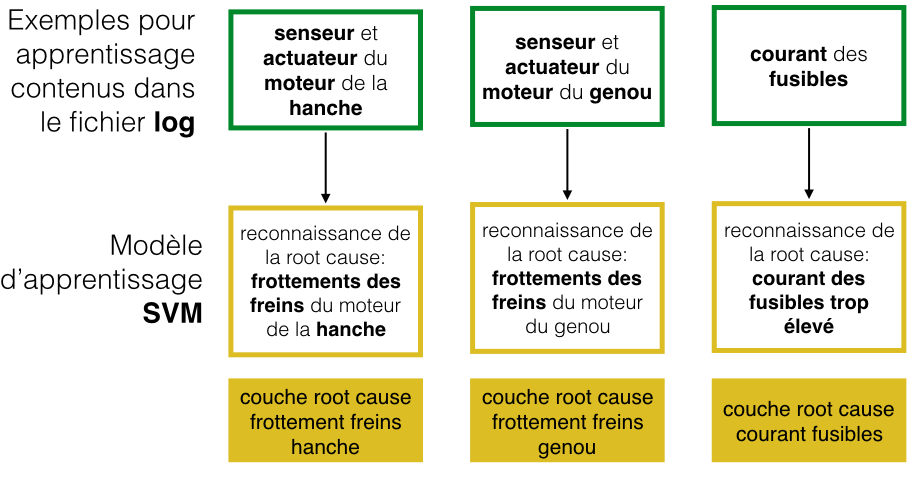
\includegraphics[height=7.5cm]{images/synoptique_root.png}
	\caption[Création des couches root cause]{Synoptique haut niveau de la création des couches root cause. Les couches root cause correspondent à des algorithmes d'apprentissage automatique que l'on entraîne à détecter la root cause à laquelle ils sont associés. Par exemple, créer la couche root cause "frottement du frein de la hanche" revient à entraîner un algorithme d'apprentissage de type SVM à partir des valeurs senseurs et actuateurs de la hanche contenues dans les différents exemples de fichiers logs générés lors de chutes de robot durant le filtering test. On réalise ce processus pour chaque couche root cause que l'on veut créer.}
	\label{fig:Creation des couches root cause}
\end{figure}

\paragraph{Utilisation du système de détection d'une root cause}
Une fois nos différentes couches root cause créées, on souhaite utiliser notre système afin de détecter la cause de la chute d'un robot (c.f. figure \ref{fig:utilisation de la couche error name}). Pour cela, on place à l'entrée de notre couche error name le fichier log que l'on souhaite analyser. Chaque couche root cause extrait du fichier log les features qui lui sont liées (e.g. la root cause "frottement des freins de la hanche" est liée aux features senseurs et actuateurs de la hanche). L'algorithme SVM de chaque couche root cause va alors émettre une décision quant à la présence ou non de la root cause dans le fichier log; Cette décision correspond à la probabilité que la root cause ait été détectée (en \%). La couche root cause ayant la probabilité la plus élevée en sortie est considérée comme la root cause (cause) ayant entrainé l'error name (i.e. la conséquence, ici la chute du robot) 

\begin{figure}[h]
	\centering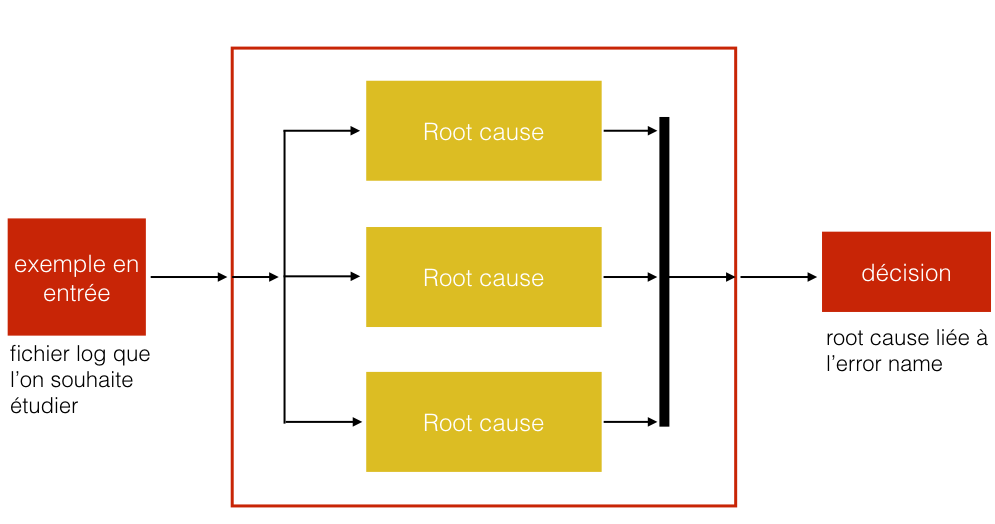
\includegraphics[height=8.5cm]{images/synoptique_error.png}
	\caption[Utilisation de la couche error name]{Synoptique haut niveau de l'utilisation de la couche error name. La couche error name contient plusieurs couches root cause. On met en entrée du système le fichier log que l'on souhaite analyser, puis chaque couche root cause va détecter la présence de la root cause à laquelle elle est rattachée. On obtient en sortie de la couche error name la root cause  ayant la plus forte probabilité d'avoir été reconnue.}
	\label{fig:utilisation de la couche error name}
\end{figure}

Chaque couche root cause peut être considérée comme un système à part entière. Le schéma fonctionnel d'une root cause (c.f. figure 	\ref{fig:Synoptique d'une couche root cause}) reprend la même structure que celui du Machine Learning (c.f. \ref{fig:Schéma fonctionnel haut niveau du Machine Learning}) car, comme dit précédemment, chaque root cause est constitué d'une instance de l'algorithme SVM. Dans la suite de notre étude de l'architecture haut niveau de la solution proposée, on s'intéressera plus particulièrement  au fonctionnement de la couche root cause car elle contient l'ensemble du traitement et de l'analyse des données.

\begin{figure}[h]
	\centering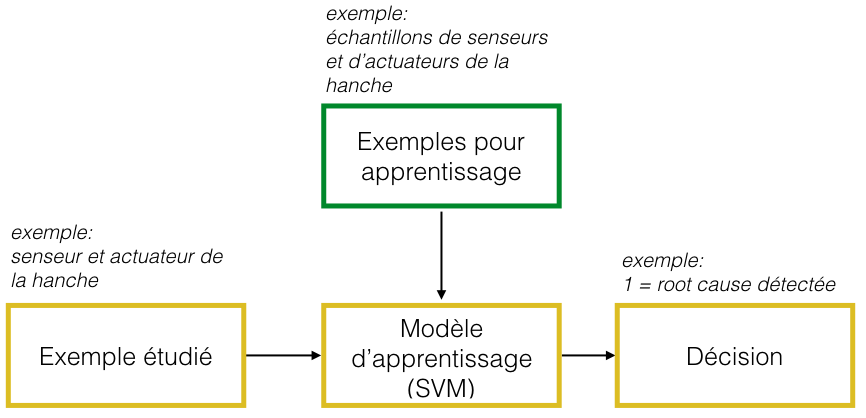
\includegraphics[height=7.4cm]{images/exemple_root.png}
	\caption[Synoptique d'une couche root cause]{Synoptique d'une couche root cause. La couche error name contient plusieurs couches root cause. On met en entrée du système le fichier log que l'on souhaite analyser, puis chaque couche root cause va détecter la présence de la root cause à laquelle elle est rattachée. On obtient en sortie de la couche error name la root cause  ayant la plus forte probabilité d'avoir été reconnue.}
	\label{fig:Synoptique d'une couche root cause}
\end{figure}

\subsection{Les exemples}
\label{Automatisation du processus d'investigation: Achitecture High Level du système proposé: Les exemples}
Les exemples sont les éléments permettant d'entraîner l'algorithme d'apprentissage automatique (c.f. partie \ref{Le Machine Learning: Généralités sur le Machine Learning: Les données}). Dans le cadre de la résolution de notre problématique, ces exemples correspondent aux données générées et enregistrées dans le fichier log lorsqu'une erreur (error name) est détectée durant le Filtering Test.

\subsubsection{Structure du fichier log}
\label{Automatisation du processus d'investigation: Achitecture High Level du système proposé: Les exemples: Structure du fichier log}
Le fichier log renferme un ensemble de données enregistrées lors de la détection d'une erreur durant le Filtering Test. Ces données correspondent aux "rythmes vitaux" du robot. Il contient par exemple l'évolution temporelle des différents actuateurs et senseurs de Pepper, la température de différentes pièces mécaniques, etc. Dans le cadre de l'entraînement de l'algorithme du Machine Learning (SVM), chacune de ces constantes correspond à une feature  (c.f. partie  \ref{Le Machine Learning: Généralités sur le Machine Learning: Définition et principe général:Lexique}). Soit le tableau \ref {tab: Extrait du contenu d'un fichier log}, un extrait du contenu d'un fichier log:

\begin{equation}
\begin{blockarray}{ccccccc}
\begin{block}{c[cccccc]}
features & HeadPitchPositionActuatorValue & HeadPitchElectricCurrentSensorValue & HipPitchPositionSensorValue & HipPitchPositionActuatorValue &  KneePitchPositionSensorValue & KneePitchPositionActuatorValue \\
t_0 & -0,404 & 0,64 & -0,023 & -0,04 & -0,008 & -0,007 \\
t_1 & -0,404 & 0,64 & -0,029 & -0,038 & -0,006 & -0,006 \\
t_3 & -0,404 & 0,576 & -0,029 & -0,033 & -0,008 & -0,012 \\
t_4 & -0,402 & 0,544 & -0,029 & -0,027 & -0,012 & -0,022 \\
t_5 & -0,401 & 0,448 & -0,029 & -0,027 & -0,015 & -0,029 \\
t_6 & -0,401 & 0,448 & -0,023 & -0,029 & -0,017 & -0,031 \\
t_7 & -0,408 & 0,096 & -0,021 & -0,031 & -0,015 & -0,032 \\
t_8 & -0,444 & 0,096 & -0,021 & -0,032 & -0,015 & 0,035 \\
t_9 & -0,486 & 0,096 & -0,021 & -0,033 & -0,017 & -0,039 \\
t_{10} & -0,523 & 0,128 & -0,021 & -0,033 & -0,018 & -0,043 \\
t_n & ... & ... & ... & ... & ... & ... \\
\end{block}
\end{blockarray}
\label {tab: Extrait du contenu d'un fichier log}
\end{equation}

Le fichier log représenté par ce tableau correspond uniquement à un seul exemple de la base de données nous servant à entrainer chacun de nos algorithmes. 
A chaque colonne du tableau correspond une feature. Chacune des lignes représente la valeur de la feature à un instant t (une ligne ne correspond pas à un exemple !). 

\subsubsection{Structure de la base de données d'exemples}
\label{Automatisation du processus d'investigation: Achitecture High Level du système proposé: Les exemples: Structure de la base de données d'exemples}
La base de donnée est composée de plusieurs exemples qui correspondent à des fichiers logs, générés lors du Filtering Test en cas de présence d'une erreur. Par exemple, dans le cadre de la construction de couche error name correspondant à la chute d'un robot, la base de donnée sera constituée de fichiers logs générés par plusieurs cas de chutes sur des robots différents. On peut représenter la structure des données de la base de données par le tableau \ref {tab: Structure de la base de données d'exemples pour l'entrainement du SVM}

\begin{equation}
\begin{blockarray}{ccccccc}
\begin{block}{c[cccccc]}
features & HeadPitchPositionActuatorValue & HeadPitchElectricCurrentSensorValue & HipPitchPositionSensorValue & HipPitchPositionActuatorValue &  KneePitchPositionSensorValue & KneePitchPositionActuatorValue \\
exemple_0 & log_0 [HeadPitchPositionActuatorValue] & log_0 [HeadPitchElectricCurrentSensorValue] & log_0 [HipPitchPositionSensorValue]& log_0 [HipPitchPositionActuatorValue] & log_0 [KneePitchPositionSensorValue] & log_0 [KneePitchPositionActuatorValue]  \\
exemple_1 & log_1 [HeadPitchPositionActuatorValue] & log_1 [HeadPitchElectricCurrentSensorValue] & log_1 [HipPitchPositionSensorValue]& log_1 [HipPitchPositionActuatorValue] & log_1 [KneePitchPositionSensorValue] & log_1 [KneePitchPositionActuatorValue]  \\
exemple_2 & log_2 [HeadPitchPositionActuatorValue] & log_2 [HeadPitchElectricCurrentSensorValue] & log_2 [HipPitchPositionSensorValue]& log_2 [HipPitchPositionActuatorValue] & log_2 [KneePitchPositionSensorValue] & log_2 [KneePitchPositionActuatorValue]  \\
exemple_3 & log_3 [HeadPitchPositionActuatorValue] & log_3 [HeadPitchElectricCurrentSensorValue] & log_3 [HipPitchPositionSensorValue]& log_3 [HipPitchPositionActuatorValue] & log_3 [KneePitchPositionSensorValue] & log_3 [KneePitchPositionActuatorValue]  \\
exemple_4 & log_4 [HeadPitchPositionActuatorValue] & log_4 [HeadPitchElectricCurrentSensorValue] & log_4 [HipPitchPositionSensorValue]& log_4 [HipPitchPositionActuatorValue] & log_4 [KneePitchPositionSensorValue] & log_4 [KneePitchPositionActuatorValue]  \\
exemple_4 & log_4 [HeadPitchPositionActuatorValue] & log_n [HeadPitchElectricCurrentSensorValue] & log_n [HipPitchPositionSensorValue]& log_n [HipPitchPositionActuatorValue] & log_n [KneePitchPositionSensorValue] & log_n [KneePitchPositionActuatorValue]  \\
\end{block}
\end{blockarray}
\label {tab: Structure de la base de données d'exemples pour l'entrainement du SVM}
\end{equation}

Tout comme la structure d'un fichier log (\ref{Automatisation du processus d'investigation: Achitecture High Level du système proposé: Les exemples: Structure du fichier log}), chaque colonne correspond à une feature. Chaque ligne de ce tableau représente un exemple et correspond à un fichier log en particulier. Cela signifie  que chaque ligne du tableau représente le contenu d'un fichier log, comme présenté dans le tableau \ref {tab: Extrait du contenu d'un fichier log}.

\subsubsection{Construction d'une couche root cause à partir de la base de données d'exemples}
\label{Automatisation du processus d'investigation: Achitecture High Level du système proposé: Les exemples: Construction d'une couche root cause à partir de la base de données d'exemples}
Lorsque l'on veut construire une nouvelle couche root cause, i.e. entraîner un nouvel algorithme d'apprentissage pour détecter la présence d'une root cause particulière dans le fichier log, on va sélectionner uniquement les features de la base de données d'exemples liées à la root cause. Par exemple, si on veut créer une nouvelle couche root cause "frottement des freins de la hanche" (lié à l'error name chute du robot), on n'utilisera que les features "HipPitchPositionSensorValue" et "HipPitchPositionActuatorValue" de notre base de données.

\subsection{Parallèle avec l'exemple de la prévision saisonnière et mise  en évidence du problème de l'évolution temporelle }
\label{Automatisation du processus d'investigation: Achitecture High Level du système proposé: Les exemples: Parallèle avec l'exemple de la prévision saisonnière}
Si on fait le parallèle avec les exemples de l'exemple "prévisions saisonnières (c.f. tableau \ref{exemples prévision saisonnière}) et ceux de notre solution (c.f. tableau \ref {tab: Structure de la base de données d'exemples pour l'entrainement du SVM}), on observe que dans les deux cas les données sont structurées en exemples et features. Cependant, dans la solution que l'on propose, les données de chaque exemple évoluent temporellement (e.g. la "HipPitchPositionSensorValue" de l'exemple 1 correspond à la colonne "HipPitchPositionSensorValue" du fichier $log_1$ qui a une évolution temporelle), alors que celles de la prévision saisonnière sont discrètes (e.g la température de l'exemple 1 est de -10\degres C, elle est discrète ) \\
Le problème est qu'on ne peut réaliser de l'apprentissage supervisé qu'avec des données discrètes. Sous leurs formes actuelles, les données de nos exemples ne peuvent donc pas servir à entrainer les algorithmes SVM de nos couches root cause. Une solution sera soumise ultérieurement en partie \ref{Automatisation du processus d'investigation: Solutions testées}


\subsection{Le modèle d'apprentissage}
\label{Automatisation du processus d'investigation: Achitecture High Level du système proposé: Le modèle d'apprentissage}
Le modèle d'apprentissage utilisé est le Support Vector Machine (SVM) avec l'utilisation de Kernels (c.f. présentation de l'algorithme partie \ref{Le Machine Learning: Les différents algorithmes: SVM}).


\subsection{La décision}
\label{Automatisation du processus d'investigation: Achitecture High Level du système proposé: La décision}
Chaque couche root cause délivre en sortie la probabilité que la root cause à laquelle elle est rattachée soit présente dans le fichier log analysé (via le SVM).



\section{Reconnaissance de motifs}
\label{Automatisation du processus d'investigation: Reconnaissance de motifs}
On souhaite réaliser de la reconnaissance de motifs grâce à l'utilisation du Machine Learning, afin de mettre en place l'automatisation du processus d'investigation. L'utilisation de cette méthode répond notamment au problème causé par l'évolution temporelle des exemples utilisés pour l'entraînement de notre système (c.f. partie \ref{Automatisation du processus d'investigation: Achitecture High Level du système proposé: Les exemples: Parallèle avec l'exemple de la prévision saisonnière}). On présente dans cette partie les différentes solutions envisagées et les raisons ayant amené à utiliser la reconnaissance de motifs. \\

Afin de simplifier le développement du système de reconnaissance de motifs, on considère dans un premier temps que chaque couche root cause est un système d'apprentissage automatique avec une seule feature en entrée. 

\subsection{Différentes approches étudiées}
\label{Automatisation du processus d'investigation: Reconnaissance de motifs: Différentes approches étudiées}
L'évolution temporelle des exemples utilisés pour l'entraînement de l'algorithme implique de prétraiter les données (c.f. partie \ref{Automatisation du processus d'investigation: Achitecture High Level du système proposé: Les exemples: Parallèle avec l'exemple de la prévision saisonnière}). Pour cela, différentes approches sont envisagées.

\subsubsection{Création de nouvelles features}
\label{Automatisation du processus d'investigation: Reconnaissance de motifs: Différentes approches étudiées: Création de nouvelles features}
On propose de créer de nouvelles features, constantes, caractéristiques des features actuelles. Dans le cadre de cette étude, on les identifiera sous l'appellation de \emph{caractéristiques simplifiées}. On peut par exemple calculer la moyenne d'une feature, sa valeur crête-à-crête, sa valeur maximum, etc. On se sert ensuite de ces nouvelles caractéristiques simplifiées pour réaliser l'entrainement de notre algorithme d'apprentissage automatique (c.f. exemple figure \ref{fig:Calcul de nouvelles features}).

\begin{figure}[h]
	\centering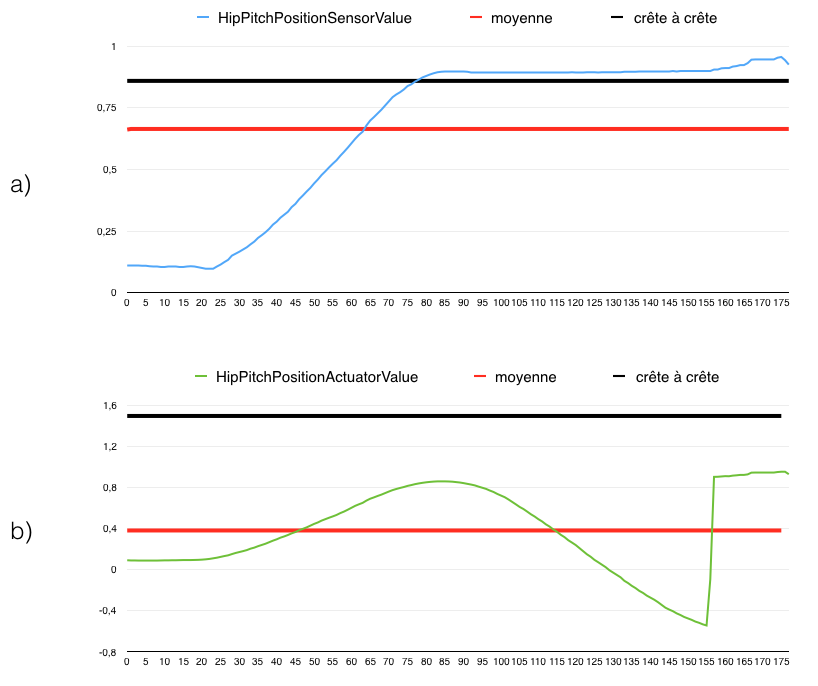
\includegraphics[height=8cm]{images/caracteristiques_simples_1.png}
	\caption[Calcul des caractéristiques simplifiées]{Calcul des caractéristiques simplifiées. Les figures a) et b) représentent respectivement l'évolution de la valeur du senseur et de l'actuateur de la hanche au cours du temps, lors de la chute d'un robot. La ligne rouge représente la valeur moyenne de chacune des features. la ligne noire correspond à la valeur crête-à-crête de chacune des features. On a ainsi réduit nos features à deux valeurs constantes. On peut donc entraîner l'algorithme d'apprentissage automatique à partir de ces caractéristiques simplifiées.}
	\label{fig:Calcul de nouvelles features}
\end{figure}


Le problème de cette approche est qu'elle réduit le nombre d'informations que contient une donnée à seulement quelques caractéristiques (e.g. moyenne et valeur crête-à-crête). Comme le démontre la figure \ref{fig:Comparaison de deux caractéristiques}, cette diminution des informations peut entrainer des risques de confusion entre différentes features, i.e. que deux features différentes peuvent avoir les mêmes caractéristiques. Or, si on souhaite utiliser cette approche dans l'architecture que l'on propose partie \ref{Automatisation du processus d'investigation: Achitecture High Level du système proposé}, le risque est que deux couches root cause soient liées à des features dont les caractéristiques sont similaires. Dans ce cas, le système est incapable de déterminer quelle root cause est responsable de l'apparition d'un error name.

\begin{figure}[h]
	\centering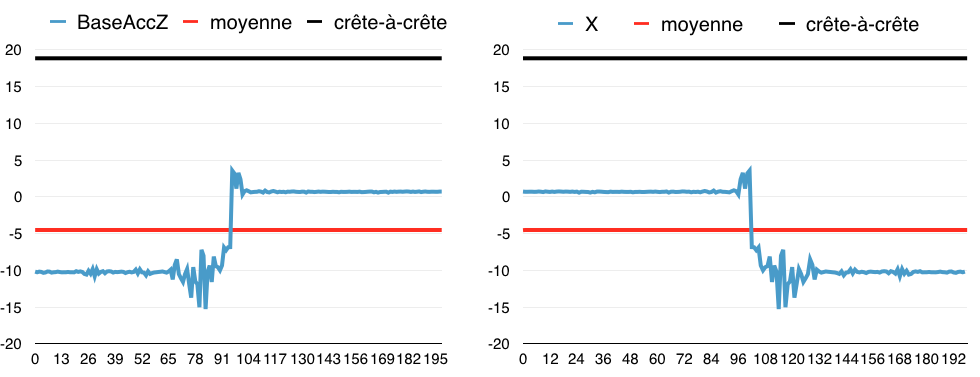
\includegraphics[height=8cm]{images/caracteristiques_simples_2.png}
	\caption[Comparaison de deux caractéristiques]{Calcul de nouvelles features. On retrouve sur la figure a) les valeurs du senseur et de l'actuateur de la hanche, ainsi que leurs caractéristiques simplifiées. Sur la figure b), on observe deux autres features et leurs caractéristiques simplifiées. On remarque que, bien qu'il s'agisse de features différentes entres les figures a) et b), ces derniers possèdent les mêmes caractéristiques simplifiées.}
	\label{fig:Comparaison de deux caractéristiques}
\end{figure}

\subsubsection{Considérer chaque unité de temps comme une feature}
\label{Automatisation du processus d'investigation: Reconnaissance de motifs: Différentes approches étudiées: Considérer chaque unité de temps comme une feature}
On propose de considérer chaque unité de temps comme une feature caractéristique de nos différents exemples. Le nombre d'entrée du système d'apprentissage automatique est donc égal au nombre d'échantillons contenus dans une donnée temporelle.

\begin{figure}[h]
	\centering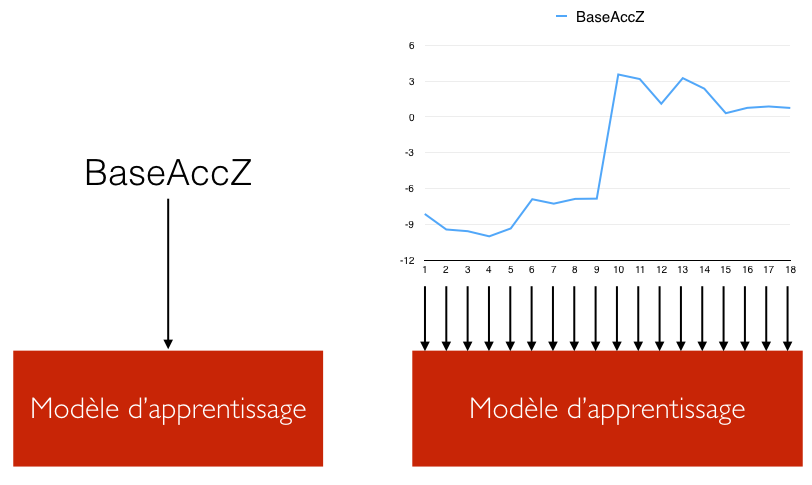
\includegraphics[height=8cm]{images/unit_tps_feature.png}
	\caption[Comparaison de deux caractéristiques]{Calcul de nouvelles features. On retrouve sur la figure a) les valeurs du senseur et de l'actuateur de la hanche, ainsi que leurs caractéristiques simplifiées. Sur la figure b), on observe deux autres features et leurs caractéristiques simplifiées. On remarque que, bien qu'il s'agisse de features différentes entres les figures a) et b), ces derniers possèdent les mêmes caractéristiques simplifiées.}
	\label{fig:Comparaison de deux caractéristiques}
\end{figure}

\subsubsection{Passage des données dans le domaine fréquentiel}
\label{Automatisation du processus d'investigation: Reconnaissance de motifs: Différentes approches étudiées: Passage des données dans le domaine fréquentiel}
Afin de supprimer l'aspect temporel des exemples, on propose de les passer dans le domaine fréquentiel. A la manière de la solution testée en partie \ref{Automatisation du processus d'investigation: Reconnaissance de motifs: Différentes approches étudiées: Considérer chaque unité de temps comme une feature} Chaque valeur fréquentielle devient alors une entrée de notre système, i.e. une feature. \\

Par exemple, on calcule la $fft$ des valeurs de l'accélération en $Z$ lors de la chute d'un robot.  

\subsubsection{Calcul de la convolution}
\label{Automatisation du processus d'investigation: Reconnaissance de motifs: Différentes approches étudiées: Calcul de la convolution}

\subsection{Concept}
\label{Automatisation du processus d'investigation: Reconnaissance de motifs: Concept}



\section{Étendre le problème à plusieurs dimensions }
\label{Automatisation du processus d'investigation: Étendre le problème à plusieurs dimensions}



\section{Difficultés notoires rencontrées}
\label{Automatisation du processus d'investigation: Difficultés notoires rencontrées}

\section{Performances de la solution}
\label{Industrialisation du produit: Performances de la solution}

